\documentclass[8 pt]{article}

\usepackage[utf8x]{inputenc}
\usepackage{dsfont}
\usepackage{amsthm}
\usepackage{amsfonts}
\usepackage{amssymb}
\usepackage{tensor}
\usepackage{mathtools}
\usepackage[T1]{fontenc}
%\usepackage[spanish]{babel}
\usepackage[cm]{fullpage}
\usepackage{graphicx}
%\usepackage{float}
\usepackage{bm}
\usepackage{setspace}
\usepackage{enumitem}
\usepackage{mdwlist}
\usepackage{parskip}
\usepackage{listings}
\usepackage{color}
%\usepackage{epstopdf}
\usepackage{tikz,datatool}
\usepackage{hyperref}
\usepackage{mathabx}
\usepackage{multicol}
\usepackage{eurosym}
\usepackage{caption}
\usepackage{pdfpages}

\newcommand{\HRule}{\rule{\linewidth}{0.5mm}}

\AtBeginDocument{
  \let\myThePage\thepage
  \renewcommand{\thepage}{\oldstylenums{\myThePage}}
}

\newcommand{\gra}{$^\text{o}$}
\newcommand{\dif}{\text{d}}
\newcommand{\avg}[1]{\left\langle #1 \right\rangle}
\newcommand{\ket}[1]{\left| #1 \right\rangle}
\newcommand{\bra}[1]{\left\langle #1 \right|}
\newcommand{\bket}[2]{\left\langle #1 \middle| #2 \right\rangle}
\newcommand{\der}[2]{\frac{\text{d} #1}{\text{d} #2}}
\newcommand{\prt}[2]{\frac{\partial #1}{\partial #2}}
\newcommand{\dert}[3]{\frac{\text{d}^#3 #1}{\text{d} #2^#3}}
\newcommand{\prtt}[3]{\frac{\partial^#3 #1}{\partial #2^#3}}
\newcommand{\dl}{\mathcal{L}}
\newcommand{\dha}{\mathcal{H}}
\newcommand{\vol}{\text{vol}}
\renewcommand{\vec}[1]{\pmb{#1}}

\DeclarePairedDelimiter\ceil{\lceil}{\rceil}
\DeclarePairedDelimiter\floor{\lfloor}{\rfloor}

\newenvironment{Figure}
  {\par\medskip\noindent\minipage{\linewidth}}
  {\endminipage\par\medskip}

\renewcommand\thesection{}

\begin{document}

\begin{minipage}{\textwidth}
    \centering
    \Large \textbf{\textsc{Homework 5: IMC assignment}}
    \vspace{0.5cm}

    \small \textsc{Francisco García Flórez, Joris van Lammeren, Wouter Varenkamp}
    \vspace{0.5cm}

    \begin{minipage}{0.8\textwidth}
      \textbf{Abstract.} In this homework we solve several exercises related to option trading proposed in the IMC guest lecture.
    \end{minipage}
\end{minipage}

\vspace{0.5cm}

\begin{multicols*}{2}

\section{Exercise 1}

To check when are the Q1 results for ING going to be published we checked the website \url{https://www.ing.com/Investor-relations.htm}, where it shows that the date is 10th of May, in 20 natural days (15 business days) as of 20th of April.

\section{Exercise 2}

Now, looking on Euronext (data attached at the end) we see the books for options expiring in April and May, right before and after the publication of the Q1 results. Since they expire the third Friday of each month, the ones in April will be done by the 21st (1 business day from today) and the ones in May by the 19th (21 business days from today).

So, using the put-call parity

\begin{equation*}
  S = C - P + Ke^{-rT} ~~,
\end{equation*}

we can compute the asset price $S$ at each time. Using only ask prices for the options (taking the point of view of someone wanting to buy) shown in the appendix, and taking the average over the strike prices, we get

\begin{align*}
  \begin{split}
    S_c &= 14.12 \\
    S_1 &= 14.11 \\
    S_2 &= 13.847
  \end{split} ~~.
\end{align*}

Here we used $r=-10bps$ per year, and we can make a few remarks. In the first place, $S_1$ is very similar to the current asset price since it expires in one day, but in $S_2$ we can see the effect of the Q1 results.

\section{Exercises 3 \& 4}

Using $S_1$ and $S_2$ we can now compute the implied volatility, again using ask prices. Since $S_1=14.11$, we will consider options at strike prices 14.00 and 14.20, and for $S_2$ these will be 13.50 and 14.00. Using Matlab's \texttt{blsimpv} function, we can compute the following implied volatilities:

\begin{align*}
  \begin{split}
    \sigma_1^- &= 28.13 \% \\
    \sigma_1^+ &= 29.80 \% \\
    \sigma_2^- &= 30.99 \% \\
    \sigma_2^+ &= 29.74 \%
  \end{split} ~~,
\end{align*}

where the superscripts $^\pm$ refer to over the forward asset price and below, respectively.

Finally, to get the volatility at the forward, we need to compute $x$ in the following equation

\begin{equation*}
  S_i = x_i K_i^+ + (1 - x_i) K_i^- \longrightarrow x_i = \frac{S_i - K_i^-}{K_i^+ - K_i^-} ~~,
\end{equation*}

and apply it to the volatilities

\begin{equation*}
  \sigma_i^f = \sqrt{(\sigma_i^+)^2 x_i + (1 - x_i) (\sigma_i^-)^2} ~~.
\end{equation*}

Following this procedure we find

\begin{align*}
  \begin{split}
    \sigma_1^f &= 28.89 \% \\
    \sigma_2^f &= 30.61 \%
  \end{split} ~~,
\end{align*}

which then we can use to compute the jump volatility.

\section{Exercise 5}

We proceed now to compute the jump volatility using the following equation

\begin{equation*}
  \sigma_{\text{jump}} = \sqrt{\sigma_{\text{after}}^2 T - \sigma_{\text{diff}}^2 (T-1)} ~~,
\end{equation*}

where we will assume $\sigma_{\text{diff}} = \sigma_1^f$, for simplification. From here, using $T=21$, we obtain a value of

\begin{equation*}
  \sigma_{\text{jump}} = 54.64 \% \longrightarrow \text{daily move} = 3.4 \% ~~.
\end{equation*}

\section{Exercise 6}

Finally we can determine what to do in this situation. Since the analyst estimates a lower daily move (2\%), we can assume that the actual movement will be less than our value, let's take 2.7\% as a more conservative value. Using these two volatilities we find that the expected asset value is going to change between 38 and 54 cents.

Since it is already too late to buy options expiring tomorrow (ask prices are higher than usual because of the Q1 results), we can buy options expiring in May, and then following a simple $\Gamma$ hedging strategy we can estimate P\&L by

\begin{equation*}
  \text{P\&L} = \Delta \delta S + \frac{1}{2}\Gamma (\delta S)^2 ~~,
\end{equation*}

so considering the $\Delta$ and $\Gamma$ values computed from the BS model shown in the last table attached, we can see that for $K$ between 14.00 and 15.00 we have $\Delta \sim 0.7$ and $\Gamma \sim 0.2$, so we can expect a P\&L between 28 and 36 cents per option.

Now, considering a volatility of 0\%, even though it's highly unlikely, our hedging strategy wouldn't work and therefore P\&L = 0. However, a change of a 10\%, again highly unlikely, would mean $\Delta \sim 0.46$ and $\Gamma \sim 0.25$, giving a P\&L of 90 cents per option, which is of course higher than our realistic estimate.

\begin{thebibliography}{1}
\raggedright
\addcontentsline{toc}{section}{Bibliography}

\bibitem{Wilmott} P. Wilmott et al, \emph{The Mathematics of Financial Derivatives}, 1995.

\end{thebibliography}

\end{multicols*}

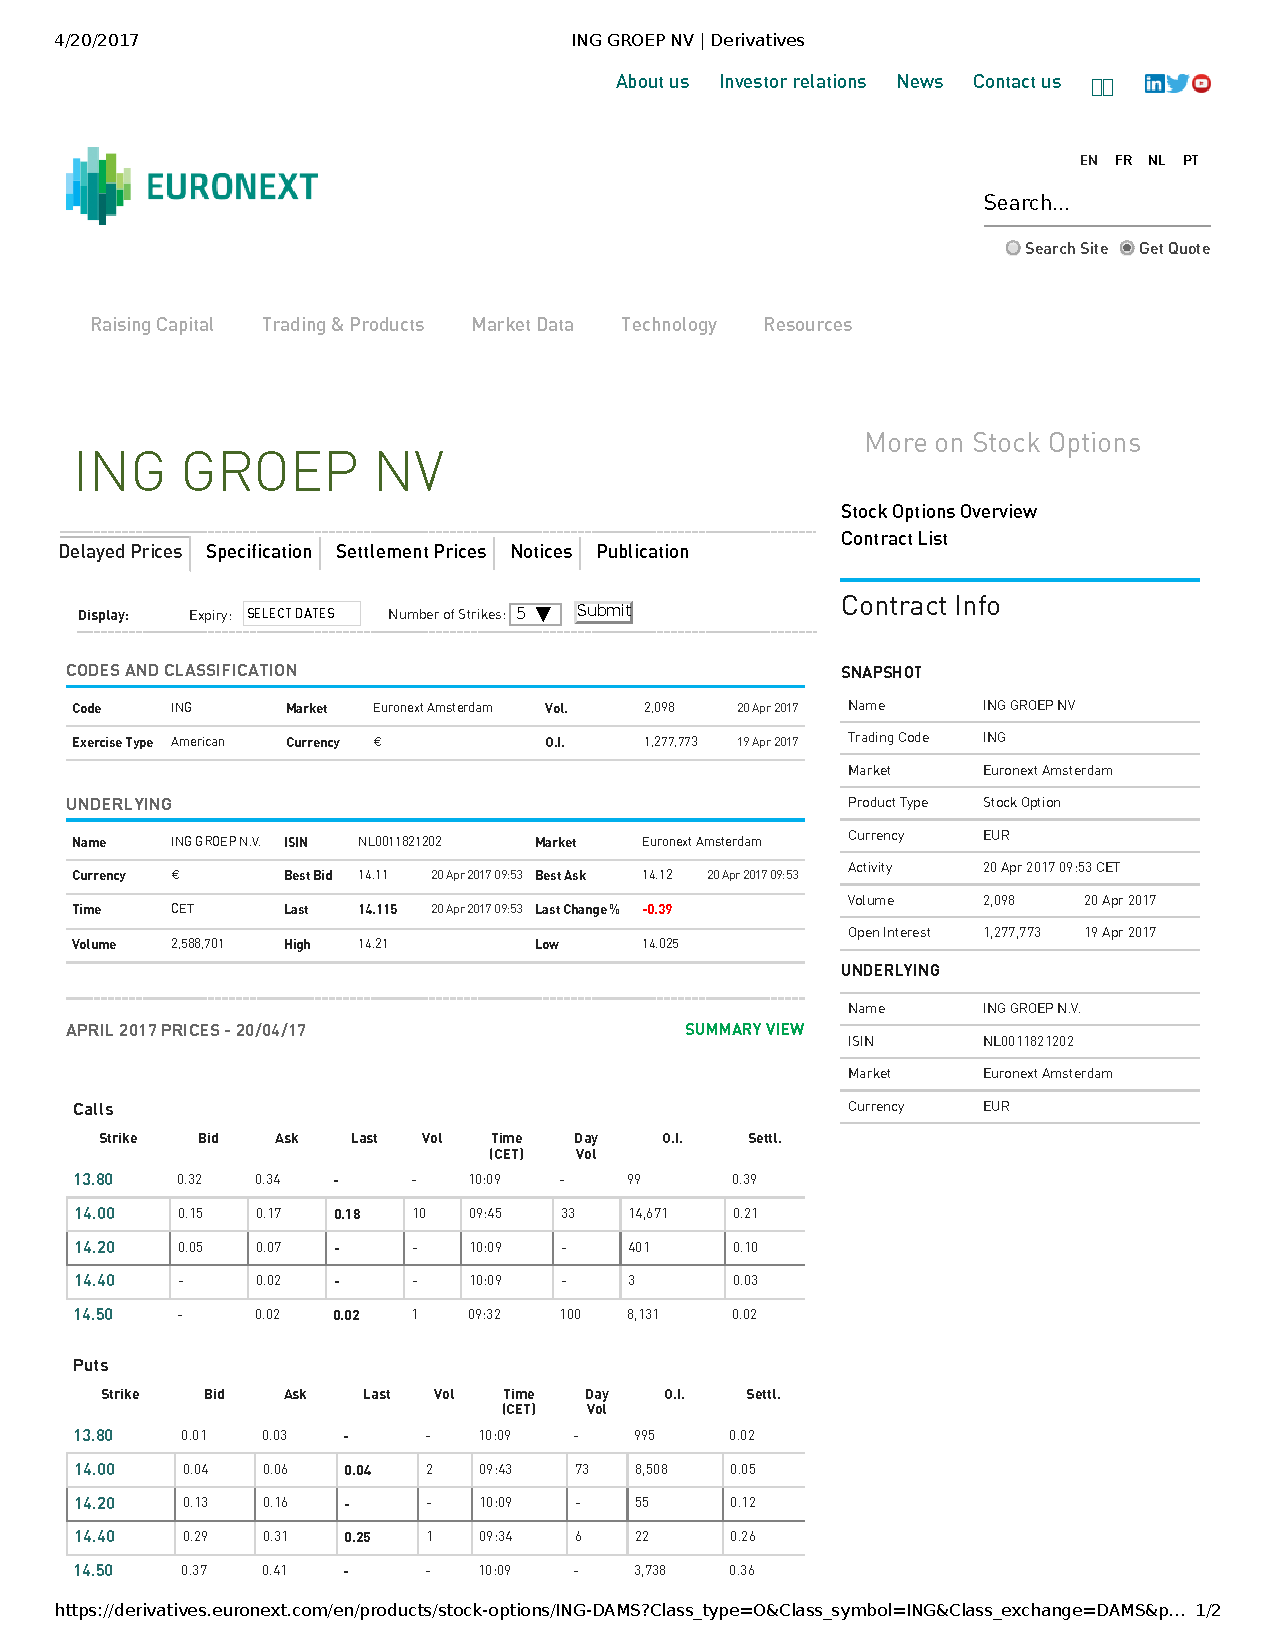
\includepdf[pages={-}]{pdf/ing_data.pdf}
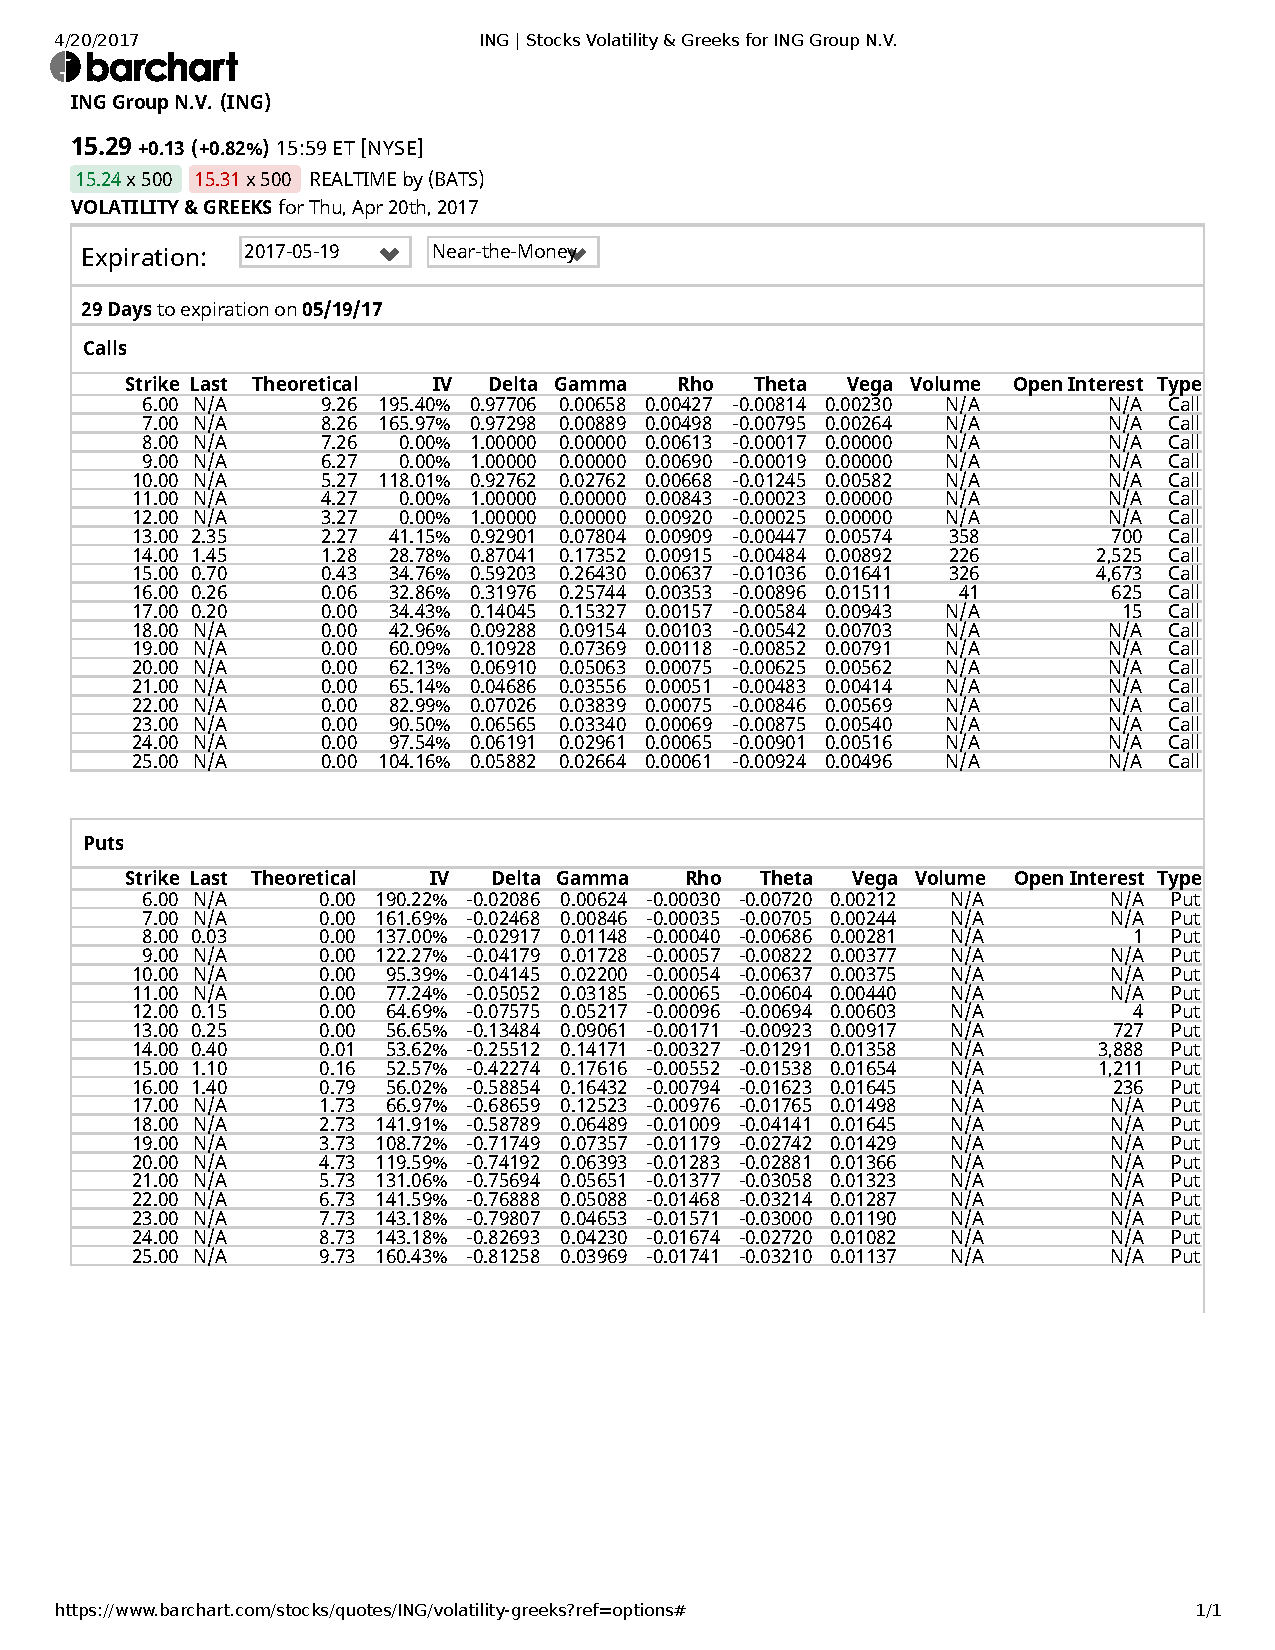
\includepdf[pages={-}]{pdf/greeks_data.pdf}

\end{document}
